Ud fra test afsnittet kan det konkluderes at alle de testede funktioner virker, som de skal. Den genetiske algoritme er dog ikke optimal, dette kan observeres på figur~\ref{fig:spredning}.
\begin{figure}[!h]
\centering
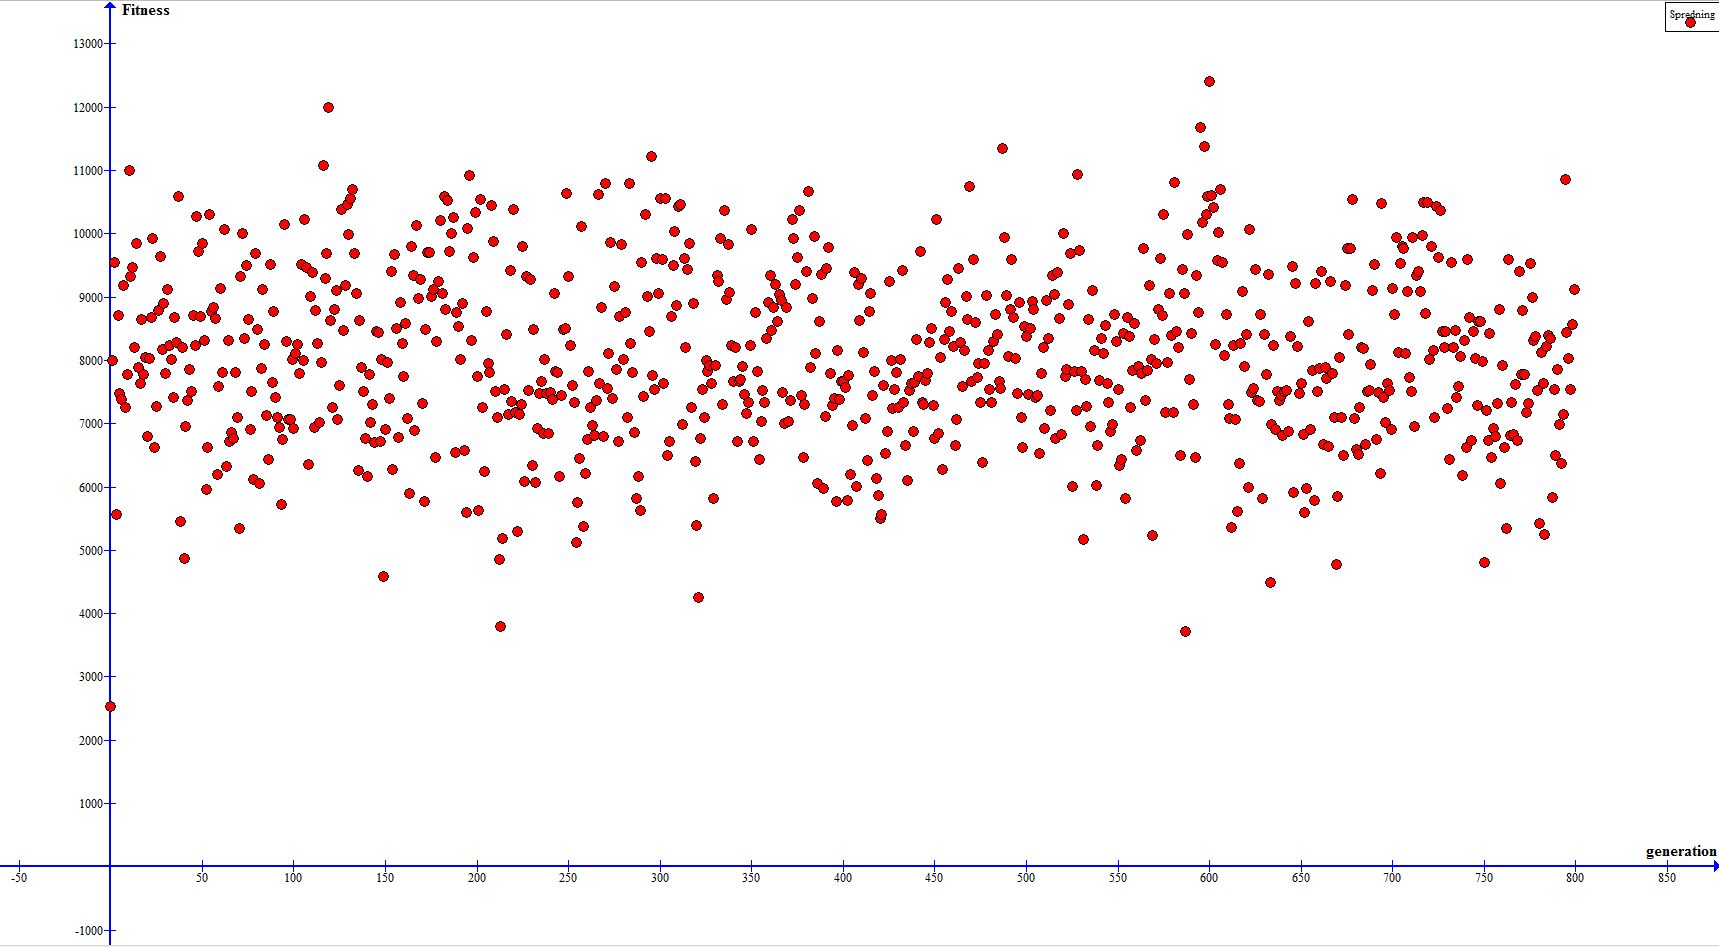
\includegraphics[scale = 0.2]{partials/graphics/spredning.png}
\caption{Graf over spredningen af fitness værdier}
\label{fig:spredning}
\end{figure}

Fitnessen er tilfældig i gennem programmet. Skemaerne bliver altså ikke bedre efter hver generation. De bliver hellere ikke dårligere, men bliver ved med at blive dannet tilfældige skemaer. Det kan skyldes, at mutationen i algoritmen er for kraftig og sker for hyppigt. Programmet er dog blevet testet med flere forskellige sandsynligheder for at mutationen opstår. Ud fra disse tests kunne det ses at sandsynligheden for at en mutation finder sted, ikke havde nogen synlig effekt på spredningsdiagrammet. Dette kan observeres på figur~\ref{fig:spredningudenmutation}.
\begin{figure}[!h]
\centering
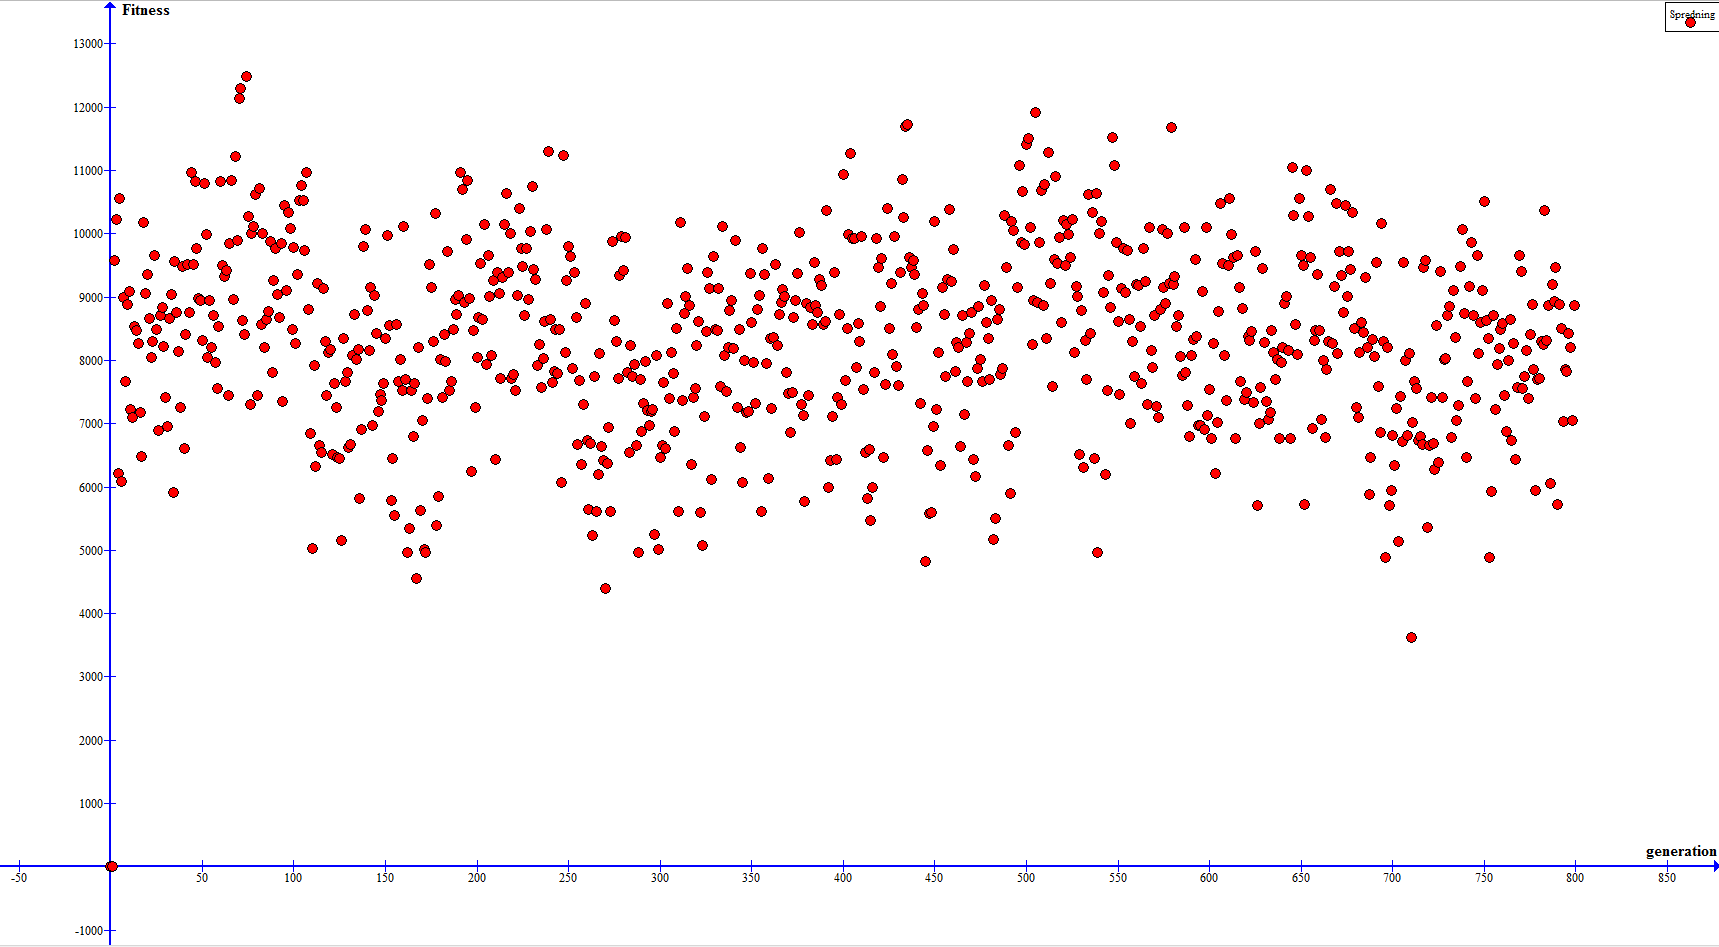
\includegraphics[scale = 0.2]{partials/graphics/spredningudenmutation.png}
\caption{Graf over spredningen af fitness værdier uden mutations funktionen}
\label{fig:spredningudenmutation}
\end{figure}

Det kunne også være, at crossoveren gør skemaerne for tilfældige. På figur~\ref{fig:spredningudencrossover} ses spredningsdiagrammet da programmet blev kørt igennem en gang uden crossoveren.
\begin{figure}[!h]
\centering
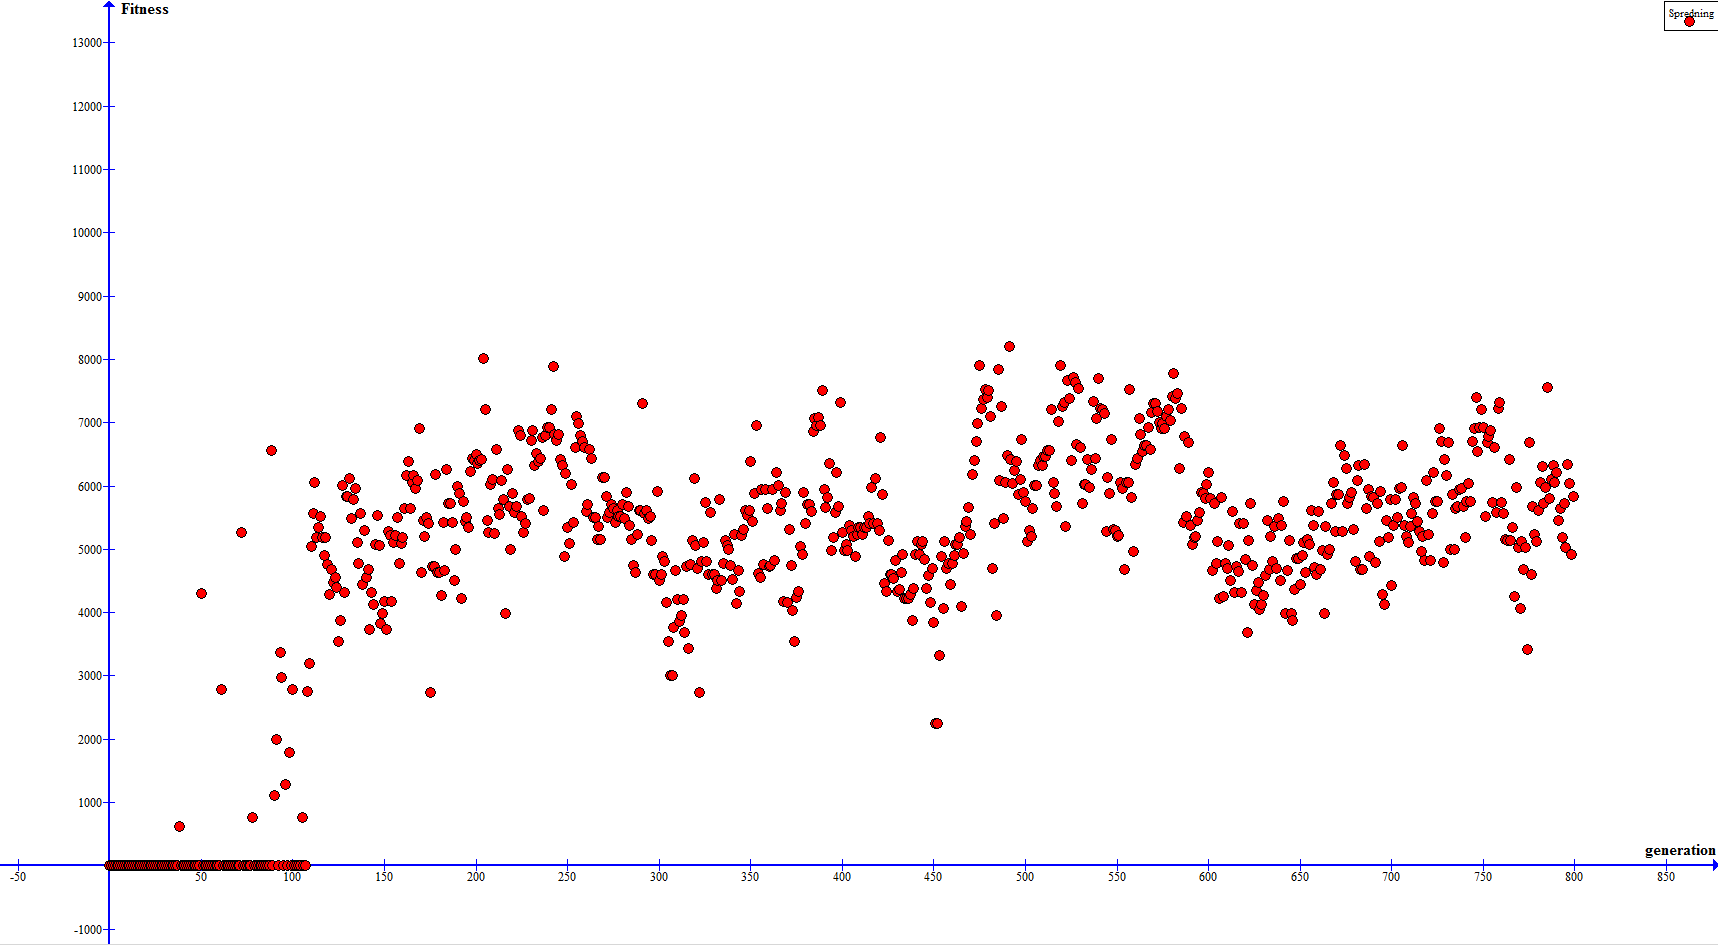
\includegraphics[scale = 0.2]{partials/graphics/spredningudencrossover.png}
\caption{Graf over spredningen af fitness værdier uden crossover funktionen}
\label{fig:spredningudencrossover}
\end{figure}
Der er altså en mere tydelig tendens i grafen, når crossoveren bliver fjernet, men kurven stiger stadig ikke konsekvent i de senere generation. Spredningen er dog mindre tilfældigt. Ud fra denne test kunne crossoverfunktionen godt være problematisk, ved at danne for tilfældige skemaer. 

På figur~\ref{fig:generationsfitness} ses det at der ikke er nogen signifikant vækst i fitnessen efter 30. generation.

\begin{figure}[!h]
\centering
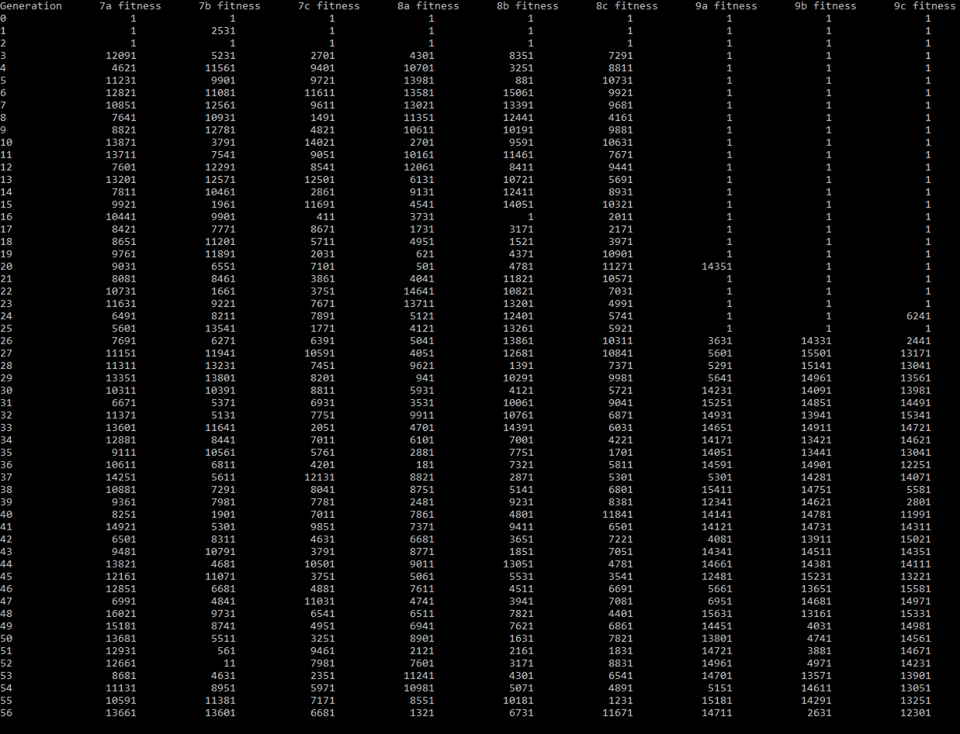
\includegraphics[scale = 0.2]{partials/graphics/generationsfitness.png}
\caption{Fitness udvikling over generationer.}
\label{fig:generationsfitness}
\end{figure}

Udover problemerne med den genetiske algoritme er der ikke det samme antal timer i alle parallelklasserne. Der er altså nogle af parallelklasserne, der har for mange lektioner af diverse fag. Det kan reguleres i fitnessværdierne, hvor meget negativ fitness det skal give at have for mange lektioner af nogle fag. I det den nuværende løsning giver det -8000 i fitnessværdi, hvis der er for mange timer.
